\subsubsection{Comprobación de algoritmos}
Primero se detallará el desarrollo para verificar que los algoritmos están correctamente diseñados, proporcionando así resultados correctos. Para esto, se ha utilizado la página web \href{https://es.planetcalc.com/1721/}{PLANETCALC}, la cual cuenta con un apartado para calcular la Distancia de Levenshtein con costos iguales para todas las operaciones. En esta página solo se entrega el resultado, por lo que se comparará este con el resultado obtenido por los algoritmos de Fuerza Bruta y Programación Dinámica.

\begin{table}[H]
    \centering
    \footnotesize
    \begin{tabular}{|c|l|l|l|l|l|}
    \hline
    \textbf{Caso de Prueba} & \textbf{Entrada \( S1 \)} & \textbf{Entrada \( S2 \)} & \textbf{PLANETCALC} & \textbf{Fuerza Bruta} & \textbf{Programación Dinámica} \\
    \hline
    1 & $"$abc$"$ & $"$abc$"$ & 0 & 0 & 0 \\
    2 & $"$ab$"$ & $"$ba$"$ & 1 & 1 & 1 \\
    3 & $"$abc$"$ & $"$acb$"$ & 2 & 1 & 1 \\
    4 & $"$abcde$"$ & $"$abcde$"$ & 0 & 0 & 0 \\
    5 & $"$abc$"$ & $"$a$"$ & 2 & 2 & 2 \\
    6 & $"$abc$"$ & $"$def$"$ & 3 & 3 & 3 \\
    7 & $"$abcd$"$ & $"$abdc$"$ & 1 & 1 & 1 \\
    8 & $"$aaa$"$ & $"$""$"$ & 3 & 3 & 3 \\
    9 & $"$""$"$ & $"$xyz$"$ & 3 & 3 & 3 \\
    10 & $"$""$"$ & $"$""$"$ & 0 & 0 & 0 \\
    11 & $"$cuadrado$"$ & $"$cuaresma$"$ & 5 & 5 & 5 \\
    12 & $"$rodilla$"$ & $"$paella$"$ & 4 & 4 & 4 \\
    13 & $"$amanda$"$ & $"$ada$"$ & 3 & 3 & 3 \\
    \hline
    \end{tabular}
    \caption{Comprobación de la efectividad de los algoritmos con algunos casos de prueba}
    \label{fig:comparacion}
\end{table}

Este paso es solo para verificar que los algoritmos están correctamente diseñados o, al menos, que arrojan el resultado correcto. Para esto, se utiliza el archivo \texttt{costos.cpp}, el cual genera los archivos \texttt{costos} con valor 1 para todas las operaciones, de la siguiente manera:

\begin{itemize}
   \item Contenido de los archivos \texttt{cost\_delete.txt} y \texttt{cost\_insert.txt} so una fila de 26 unos, cada uno representa una letra.
   \item El contenido de los archivos \texttt{cost\_replace.txt} y \texttt{cost\_transpose.txt} son matrices simétrics de \texttt{26x26} que representan el valor de cambiar una letra por otra con un 1. 
\end{itemize}

Se puede observar en el Cuadro \ref{fig:comparacion} que los valores obtenidos son bastante similares (caso 3 varia porque se realiza una transposición), pero esto puede resultar engañoso, ya que la página PLANETCALC utiliza el cálculo original de la Distancia de Levenshtein, donde solo se consideran las operaciones de inserción, eliminación y reemplazo. Es por esto que estas medidas solo se tomaron como referencia para verificar los algoritmos.

\subsubsection{Soluciones encontradas}
Para generar los costos variables, los cuales son requisitos dentro del problema a resolver, se creó el archivo \texttt{random-costos.cpp}, el cual genera los costos asignando un valor aleatorio de 1 a 10 para cada operación. Los costos utilizados pueden verse en el repositorio de Github, aquí están los enlaces:

\begin{itemize}
    \begin{minipage}{0.5\textwidth}
        \item \href{https://github.com/luphin/Tarea2y3Algoritmos-FB-PD/blob/main/codigos/cost_delete.txt}{delete}
        \item \href{https://github.com/luphin/Tarea2y3Algoritmos-FB-PD/blob/main/codigos/cost_insert.txt}{insert}
    \end{minipage}%
    \begin{minipage}{0.5\textwidth}
        \item \href{https://github.com/luphin/Tarea2y3Algoritmos-FB-PD/blob/main/codigos/cost_replace.txt}{replace}
        \item \href{https://github.com/luphin/Tarea2y3Algoritmos-FB-PD/blob/main/codigos/cost_transpose.txt}{transpose}
    \end{minipage}
\end{itemize}


Al ejecutar el \verb|main.cpp| con estos costos, los resultados obtenidos se pueden evidenciar en el archivo \verb|resultados.txt|, en el cual se encuentra que:

\begin{table}[H]
    \centering
    \footnotesize
    \begin{tabular}{|c|l|l|l|l|}
    \hline
    \textbf{Caso de Prueba} & \textbf{Entrada \( S1 \)} & \textbf{Entrada \( S2 \)} & \textbf{Distancia MIN (FB)} & \textbf{Distancia MIN(PD)} \\
    \hline
    1 & $"$abc$"$ & $"$abc$"$ & 0 & 0 \\
    2 & $"$ab$"$ & $"$ba$"$ & 3 & 3 \\
    3 & $"$abc$"$ & $"$acb$"$ & 2 & 2 \\
    4 & $"$abcde$"$ & $"$abcde$"$ & 0 & 0 \\
    5 & $"$abc$"$ & $"$a$"$ & 4 & 4 \\
    6 & $"$abc$"$ & $"$def$"$ & 14 & 14 \\
    7 & $"$abcd$"$ & $"$abdc$"$ & 2 & 2 \\
    8 & $"$aaa$"$ & $"$""$"$ & 6 & 6 \\
    9 & $"$""$"$ & $"$xyz$"$ & 15 & 15 \\
    10 & $"$""$"$ & $"$""$"$ & 0 & 0 \\
    11 & $"$cuadrado$"$ & $"$cuaresma$"$ & 15 & 15 \\
    12 & $"$rodilla$"$ & $"$paella$"$ & 20 & 20 \\
    13 & $"$amanda$"$ & $"$ada$"$ & 13 & 13 \\
    \hline
    \end{tabular}
    \caption{Resultados (distancia MIN = costo MIN)}
    \label{fig:resultados}
\end{table}

\begin{figure}[H]
    \centering
    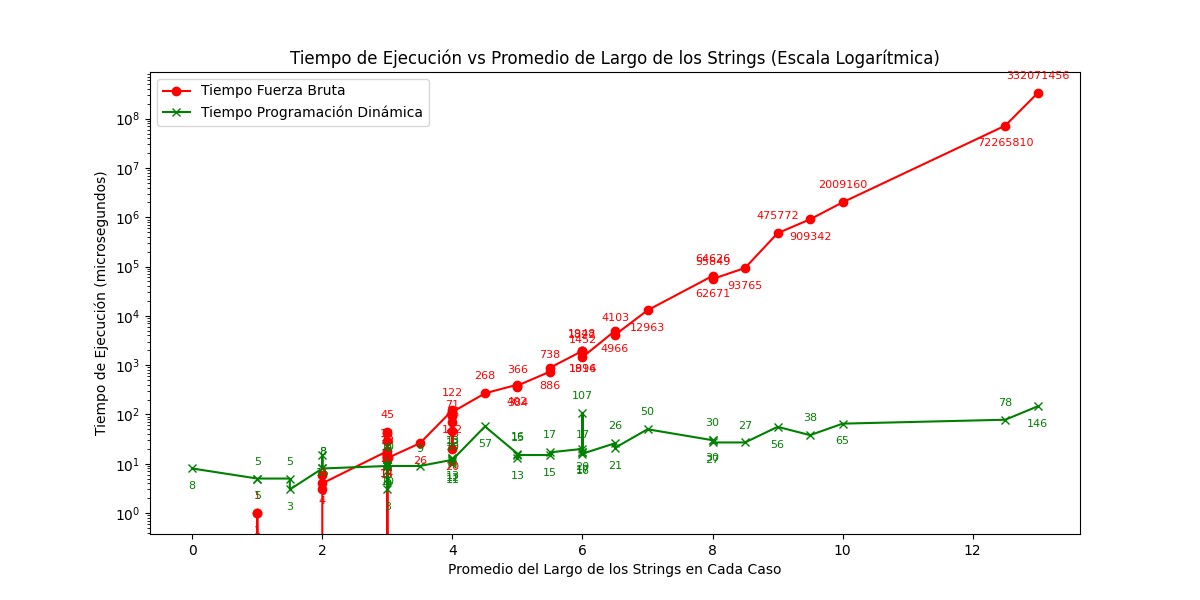
\includegraphics[width=1\textwidth]{images/Figure_1.png}
    \caption{Gráfica obtenida con los resultados de las pruebas.}
    \label{fig:tiempo}
\end{figure}
\begin{figure}[H]
    \centering
    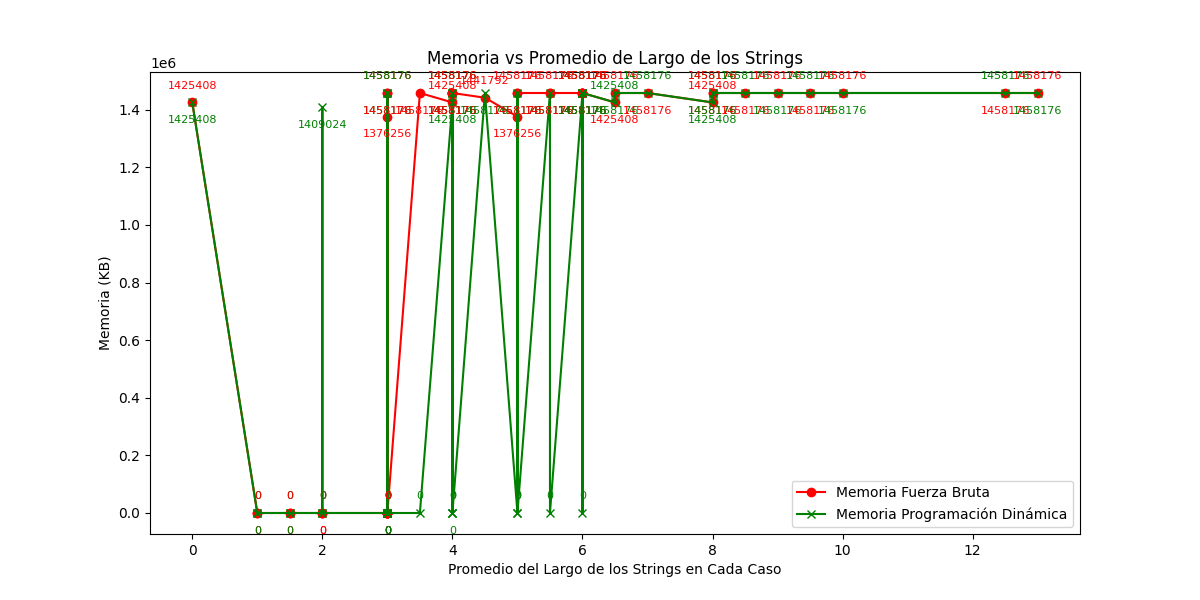
\includegraphics[width=1\textwidth]{images/Figure_2.png}
    \caption{Gráfica obtenida con resultados de las pruebas.}
    \label{fig:memoria}
\end{figure}

La Figura \ref{fig:tiempo} se genera a partir de los resultados de los casos de prueba registrados en el archivo \href{https://github.com/luphin/Tarea2y3Algoritmos-FB-PD/blob/main/codigos/resultados.txt}{resultados.txt}. En ella, se observa el comportamiento de los algoritmos en función del tiempo que tardan según el promecio de longitud de las cadenas de entrada, además de cómo influye la estructura de dichas cadenas. A medida que aumenta el promedio de la suma de las longitudes de las cadenas, el tiempo de ejecución incrementa de manera más pronunciada en el algoritmo de Fuerza Bruta, mientras que el algoritmo de Programación Dinámica muestra un cambio más controlado, corroborando el análisis aisntótico realizado.

También se intentó registrar la memoria utilizada por cada función para resolver el problema, pero la implementación no fue correcta, ya que registraba todas las ejecuciones de los algoritmos, incluidas aquellas que no afectaban el resultado final. Esto se realizó mediante un hilo que se ejecutaba en paralelo con el archivo \texttt{main.cpp}, consultando la memoria utilizada cada 10 milisegundos y almacenándola en una variable global. Durante estas pruebas, no se ejecutó ningún otro programa para evitar interferencias en los resultados. La memoria utilizada se presenta en la Figura \ref{fig:memoria}; Sin embargo, debido a que no se obtuvo un registro correcto de las operaciones realizadas por los algoritmos, el archivo \texttt{operaciones.txt} registraba una gran cantidad de líneas de operaciones, lo que resultaba en un archivo extremadamente extenso y pesado para ser cargado en GitHub. Por esta razón, el archivo disponible en el repositorio corresponde a una ejecución con menos casos de prueba, lo cual permite evidenciar de manera más clara los datos que se generan.


% Autor
% Luis Zegarra Stuardo
% 202073628-6
% Tarea 2 y 3
% Algoritmos y Complejidad 2024-2